% !TEX root = ../main.tex
\begin{tikzpicture}[line width=1pt,node distance=14mm ,main/.style = {draw, rectangle},scale=1] 

    \node[scale=.8] at (-4,1){$\textup{PerfMatch}[b,\{x_1,x_4\}]$};
       \node[main] at (-4,-0.5) (9) {
   \begin{tikzpicture}[line width=1pt,node distance=14mm ,main/.style = {draw, circle},scale=1] 
   \node[main,fill=red!40!white,densely dashed] at (0,1) (x1) {\texttt{$x_1$}};
   \node[main,color=black] at (1,1) (x2) {\texttt{$x_2$}};
       \node[main,color=black] at (0,0) (x3) {\texttt{$x_3$}};
       \node[main,fill=red!40!white,densely dashed] at (1,0) (x4) {\texttt{$x_4$}};
      \draw  (x1) -- (x2);
       \draw (x1) -- (x3);
      \draw (x2) -- (x3);
      \draw (x3) -- (x4);
   \end{tikzpicture}
       };
       
    \node[scale=.8] at (0,5.5){$\textup{PerfMatch}[c_1,\{x_1,x_4\}\cup \{x_2,x_3\}]$};
       \node[main] at (0,4) (8) {
   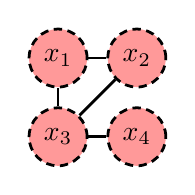
\begin{tikzpicture}[line width=1pt,node distance=14mm ,main/.style = {draw, circle},scale=1] 
   \node[main,fill=red!40!white,densely dashed] at (0,1) (x1) {\texttt{$x_1$}};
   \node[main,fill=red!40!white,densely dashed] at (1,1) (x2) {\texttt{$x_2$}};
       \node[main,fill=red!40!white,densely dashed] at (0,0) (x3) {\texttt{$x_3$}};
       \node[main,fill=red!40!white,densely dashed] at (1,0) (x4) {\texttt{$x_4$}};
      \draw (x1) -- (x2);
       \draw (x1) -- (x3);
      \draw (x2) -- (x3);
      \draw (x3) -- (x4);
   \end{tikzpicture}
   };
   
    \node[scale=3] at (2,4){$\cdot$};
   
    \node[scale=.8] at (4,5.5){$\textup{PerfMatch}[c_2,\{x_1,x_4\}\cup \{\}]$};
   \node[main] at (4,4) (8) {
   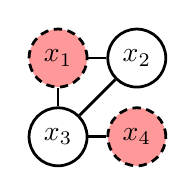
\begin{tikzpicture}[line width=1pt,node distance=14mm ,main/.style = {draw, circle},scale=1] 
   \node[main,fill=red!40!white,densely dashed] at (0,1) (x1) {\texttt{$x_1$}};
   \node[main,color=black] at (1,1) (x2) {\texttt{$x_2$}};
       \node[main,color=black] at (0,0) (x3) {\texttt{$x_3$}};
       \node[main,fill=red!40!white,densely dashed] at (1,0) (x4) {\texttt{$x_4$}};
      \draw (x1) -- (x2);
       \draw (x1) -- (x3);
      \draw (x2) -- (x3);
      \draw (x3) -- (x4);
   \end{tikzpicture}
   };
   
    \node[scale=.8] at (0,2.5){$\textup{PerfMatch}[c_1,\{x_1,x_4\}\cup \{x_3\}]$};
   \node[main] at (0,1) (8) {
   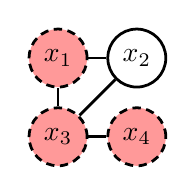
\begin{tikzpicture}[line width=1pt,node distance=14mm ,main/.style = {draw, circle},scale=1] 
   \node[main,fill=red!40!white,densely dashed] at (0,1) (x1) {\texttt{$x_1$}};
   \node[main,color=black] at (1,1) (x2) {\texttt{$x_2$}};
       \node[main,fill=red!40!white,densely dashed] at (0,0) (x3) {\texttt{$x_3$}};
       \node[main,fill=red!40!white,densely dashed] at (1,0) (x4) {\texttt{$x_4$}};
      \draw (x1) -- (x2);
       \draw (x1) -- (x3);
      \draw (x2) -- (x3);
      \draw (x3) -- (x4);
   \end{tikzpicture}
   };
   
    \node[scale=3] at (2,1){$\cdot$};
   
    \node[scale=.8] at (4,2.5){$\textup{PerfMatch}[c_2,\{x_1,x_4\}\cup \{x_2\}]$};
   \node[main] at (4,1) (8) {
   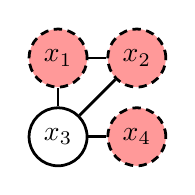
\begin{tikzpicture}[line width=1pt,node distance=14mm ,main/.style = {draw, circle},scale=1] 
   \node[main,fill=red!40!white,densely dashed] at (0,1) (x1) {\texttt{$x_1$}};
   \node[main,fill=red!40!white,densely dashed] at (1,1) (x2) {\texttt{$x_2$}};
       \node[main,color=black] at (0,0) (x3) {\texttt{$x_3$}};
       \node[main,fill=red!40!white,densely dashed] at (1,0) (x4) {\texttt{$x_4$}};
      \draw (x1) -- (x2);
       \draw (x1) -- (x3);
      \draw (x2) -- (x3);
      \draw (x3) -- (x4);
   \end{tikzpicture}
   };
   
    \node[scale=.8] at (0,-0.5){$\textup{PerfMatch}[c_1,\{x_1,x_4\}\cup \{x_2\}]$};
   \node[main] at (0,-2) (8) {
   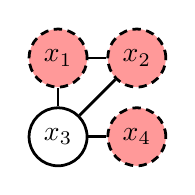
\begin{tikzpicture}[line width=1pt,node distance=14mm ,main/.style = {draw, circle},scale=1] 
   \node[main,fill=red!40!white,densely dashed] at (0,1) (x1) {\texttt{$x_1$}};
   \node[main,fill=red!40!white,densely dashed] at (1,1) (x2) {\texttt{$x_2$}};
       \node[main,color=black] at (0,0) (x3) {\texttt{$x_3$}};
       \node[main,fill=red!40!white,densely dashed] at (1,0) (x4) {\texttt{$x_4$}};
      \draw (x1) -- (x2);
       \draw (x1) -- (x3);
      \draw (x2) -- (x3);
      \draw (x3) -- (x4);
   \end{tikzpicture}
   };
   
    \node[scale=3] at (2,-2){$\cdot$};
   
    \node[scale=.8] at (4,-0.5){$\textup{PerfMatch}[c_2,\{x_1,x_4\}\cup \{x_3\}]$};
   \node[main] at (4,-2) (8) {
   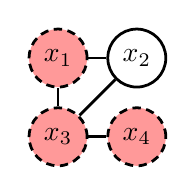
\begin{tikzpicture}[line width=1pt,node distance=14mm ,main/.style = {draw, circle},scale=1] 
   \node[main,fill=red!40!white,densely dashed] at (0,1) (x1) {\texttt{$x_1$}};
   \node[main,color=black] at (1,1) (x2) {\texttt{$x_2$}};
       \node[main,fill=red!40!white,densely dashed] at (0,0) (x3) {\texttt{$x_3$}};
       \node[main,fill=red!40!white,densely dashed] at (1,0) (x4) {\texttt{$x_4$}};
      \draw (x1) -- (x2);
       \draw (x1) -- (x3);
      \draw (x2) -- (x3);
      \draw (x3) -- (x4);
   \end{tikzpicture}
   };
   
    \node[scale=.8] at (0,-3.5){$\textup{PerfMatch}[c_1,\{x_1,x_4\}\cup \{\}]$};
   \node[main] at (0,-5) (8) {
   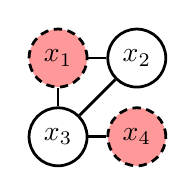
\begin{tikzpicture}[line width=1pt,node distance=14mm ,main/.style = {draw, circle},scale=1] 
   \node[main,fill=red!40!white,densely dashed] at (0,1) (x1) {\texttt{$x_1$}};
   \node[main,color=black] at (1,1) (x2) {\texttt{$x_2$}};
       \node[main,color=black] at (0,0) (x3) {\texttt{$x_3$}};
       \node[main,fill=red!40!white,densely dashed] at (1,0) (x4) {\texttt{$x_4$}};
      \draw (x1) -- (x2);
       \draw (x1) -- (x3);
      \draw (x2) -- (x3);
      \draw (x3) -- (x4);
   \end{tikzpicture}
   };
   
    \node[scale=3] at (2,-5){$\cdot$};
   
     \node[scale=.8] at (4,-3.5){$\textup{PerfMatch}[c_2,\{x_1,x_4\}\cup \{x_2,x_3\}]$};
   \node[main] at (4,-5) (8) {
   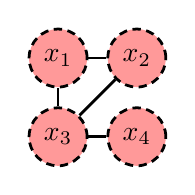
\begin{tikzpicture}[line width=1pt,node distance=14mm ,main/.style = {draw, circle},scale=1] 
   \node[main,fill=red!40!white,densely dashed] at (0,1) (x1) {\texttt{$x_1$}};
   \node[main,fill=red!40!white,densely dashed] at (1,1) (x2) {\texttt{$x_2$}};
       \node[main,fill=red!40!white,densely dashed] at (0,0) (x3) {\texttt{$x_3$}};
       \node[main,fill=red!40!white,densely dashed] at (1,0) (x4) {\texttt{$x_4$}};
      \draw (x1) -- (x2);
       \draw (x1) -- (x3);
      \draw (x2) -- (x3);
      \draw (x3) -- (x4);
   \end{tikzpicture}
   };
   
       \draw [decorate,decoration={brace,amplitude=10}] (-2,-5) -- (-2,4) node [black,midway,xshift=-0.6cm] {};
   
       %\draw [->](-2,3.5) -- (-3,2.5);
       %\draw [->](-2,1) -- (-3,0.5);
       %\draw [->](-2,-2) -- (-3,-1.5);
       %\draw [->](-2,-4.5) -- (-3,-3.5);
       %\draw [->](3.5,-2.5) -- (5,-3);
       %\draw [->](3.5,-5) -- (5,-4.5);
       %\draw [->](3.5,-7.5) -- (5,-6);
       %\node[text width=6cm] at (2,-2){$\DP[i,c]$};
       %\node[text width=6cm] at (5.5,-2){$\DP[i,c+\{x_4\to \texttt{gray/dotted}]$};
      
   \end{tikzpicture}